\documentclass[pdf, aspectratio=169]{beamer}\usepackage[]{graphicx}\usepackage[]{color}
% maxwidth is the original width if it is less than linewidth
% otherwise use linewidth (to make sure the graphics do not exceed the margin)
\makeatletter
\def\maxwidth{ %
  \ifdim\Gin@nat@width>\linewidth
    \linewidth
  \else
    \Gin@nat@width
  \fi
}
\makeatother

\definecolor{fgcolor}{rgb}{0.345, 0.345, 0.345}
\newcommand{\hlnum}[1]{\textcolor[rgb]{0.686,0.059,0.569}{#1}}%
\newcommand{\hlstr}[1]{\textcolor[rgb]{0.192,0.494,0.8}{#1}}%
\newcommand{\hlcom}[1]{\textcolor[rgb]{0.678,0.584,0.686}{\textit{#1}}}%
\newcommand{\hlopt}[1]{\textcolor[rgb]{0,0,0}{#1}}%
\newcommand{\hlstd}[1]{\textcolor[rgb]{0.345,0.345,0.345}{#1}}%
\newcommand{\hlkwa}[1]{\textcolor[rgb]{0.161,0.373,0.58}{\textbf{#1}}}%
\newcommand{\hlkwb}[1]{\textcolor[rgb]{0.69,0.353,0.396}{#1}}%
\newcommand{\hlkwc}[1]{\textcolor[rgb]{0.333,0.667,0.333}{#1}}%
\newcommand{\hlkwd}[1]{\textcolor[rgb]{0.737,0.353,0.396}{\textbf{#1}}}%
\let\hlipl\hlkwb

\usepackage{framed}
\makeatletter
\newenvironment{kframe}{%
 \def\at@end@of@kframe{}%
 \ifinner\ifhmode%
  \def\at@end@of@kframe{\end{minipage}}%
  \begin{minipage}{\columnwidth}%
 \fi\fi%
 \def\FrameCommand##1{\hskip\@totalleftmargin \hskip-\fboxsep
 \colorbox{shadecolor}{##1}\hskip-\fboxsep
     % There is no \\@totalrightmargin, so:
     \hskip-\linewidth \hskip-\@totalleftmargin \hskip\columnwidth}%
 \MakeFramed {\advance\hsize-\width
   \@totalleftmargin\z@ \linewidth\hsize
   \@setminipage}}%
 {\par\unskip\endMakeFramed%
 \at@end@of@kframe}
\makeatother

\definecolor{shadecolor}{rgb}{.97, .97, .97}
\definecolor{messagecolor}{rgb}{0, 0, 0}
\definecolor{warningcolor}{rgb}{1, 0, 1}
\definecolor{errorcolor}{rgb}{1, 0, 0}
\newenvironment{knitrout}{}{} % an empty environment to be redefined in TeX

\usepackage{alltt}
% \documentclass[pdf, aspectratio=1610]{beamer}
%\setbeamersize{text margin left=2cm, text margin right=2cm}
\setbeamersize{text margin left=1.5cm, text margin right=1.5cm}
% \documentclass[pdf]{beamer}
% \usefonttheme[onlymath]{serif} % For serif font in math mode

\usepackage[italian]{babel} %La data compare in italiano e la divisione in sillabe diventa quella italiana
\usepackage[utf8]{inputenc} %Permette di scrivere le lettere accentate
\usepackage[T1]{fontenc}
\usepackage{hyperref} %Permette di inserire i collegamenti ipertestuali
\usepackage{url}			        %Permette di inserire i link urle
\usepackage{amsmath,amssymb}
\usepackage{multirow} % Per usare il multirow nei tabular

\usepackage{graphicx} %Serve per inserire le immagini
\usepackage{xcolor}
%\usepackage{subfigure}
\usepackage{caption}
\usepackage{subcaption}

%Disegni LaTeX
\usepackage{tikz}
\usetikzlibrary{shapes}
%\usetikzlibrary{shapes,snakes}
%\usetikzlibrary{trees}
\newcommand{\ImageWidth}{11cm}
\usetikzlibrary{decorations.pathreplacing, positioning, arrows.meta}
\usepackage{pgfplots,siunitx}
\usepackage{adjustbox}

\pgfplotsset{compat=1.9}
\usepgfplotslibrary{units}

%%%%%%%%%%%%%%%%%%%%%%%%%%%%%%%%%%%%%%%%%%%%%%%%%%%%%%%%%%%%%%%%%%%%%%%%%%%%%%%%%%%%%%%%%%%%%%%%%%%%%

%Nuovi comandi
\newcommand{\magnitude}[1]{\left\lVert #1 \right\rVert}
\DeclareMathOperator*{\argmin}{arg\,min}  % Declaring operator argmin
\DeclareMathOperator*{\argmax}{arg\,max}  % Declaring operator argmax

%%%%%%%%%%%%%%%%%%%%%%%%%%%%%%%%%%%%%%%%%%%%%%%%%%%%%%%%%%%%%
\usetheme{Pittsburgh}
%\usetheme{CambridgeUS}
%\mode<presentation>{\usetheme{Boadilla}}
%singapore

%\useoutertheme[right]{sidebar}
% \usecolortheme{seahorse}
\usecolortheme{beaver}
%\usecolortheme{dolphin}
%\definecolor{UBCblue}{rgb}{0.04706, 0.13725, 0.26667} % UBC Blue (primary)
%\usecolortheme[named=UBCblue]{structure}
%\usecolortheme[named=UBCblue]{seahorse}
%\usecolortheme{structure}

\usefonttheme{professionalfonts}
\setbeamercovered{dynamic}

\usepackage{amsthm}
\theoremstyle{definition}
\newtheorem{definizione}{Definizione}[section]
%\theoremstyle{plain}
%\newtheorem{teorema}{Teorema}


\definecolor{amber(sae/ece)}{rgb}{1.0, 0.49, 0.0}
\definecolor{ao(english)}{rgb}{0.0, 0.5, 0.0}
\definecolor{myblue}{RGB}{0,82,155}

\title{Application of GLM Advancements \\ to Non-Life Insurance Pricing}
%\subtitle{}
\author{Leonardo Stincone}

\date{10 Maggio 2021}
\institute[units]{Università degli Studi di Trieste}

\logo{

\includegraphics[width=10mm, height=10mm]{figures/university-logo.png}
}


% % For table of contents positioning
% % \newsavebox{\longestsec}% Box to save longest sectional heading
% \usepackage{varwidth}    
% \usepackage{etoolbox}
% \makeatletter
% %\patchcmd{\beamer@sectionintoc}{\vskip1.5em}{\vskip0.5em}{}{}
% \patchcmd{\beamer@sectionintoc}{%
%   \hbox{\vbox{%
%     \def\beamer@breakhere{\\}%
%     \beamer@tocact{\ifnum\c@section=#1\beamer@toc@cs\else\beamer@toc@os\fi}{section in toc}}}%
% }{%
%   \hbox{%
%     \def\beamer@breakhere{}%
%     \beamer@tocact{\ifnum\c@section=#1\beamer@toc@cs\else\beamer@toc@os\fi}{section in toc}}%
% }{}{}
% \makeatother    

% \newcommand\Closer[2][1cm]{%
% \makebox[\linewidth][c]{%
%   \begin{minipage}{\dimexpr\textwidth+#1\relax}
%   \raggedright#2
%   \end{minipage}%
%   }%
% }


\setbeamertemplate{section in toc}[sections numbered]    



% Insert table of content at the beginning of each section
\AtBeginSection[]
{
  \begin{frame}
    \frametitle{Table of Contents}
    
    \tableofcontents[currentsection]
    
    % \begin{center}
    %   \begin{varwidth}{\textwidth}
    %     \tableofcontents[currentsection]
    %   \end{varwidth}
    % \end{center}
  \end{frame}
}



%%%%%%%%%%%%%%%%%%%%%%%%%%%%%%%%%%%%%%%%%%%%%%%%%%%%%%%%%%%%%%%%%%%%%%%%%%%%%%%%%%%%%%%%%%%%%%%%%%%%%
%%%%%%%%%%%%%%%%%%%%%%%%%%%%%%%%%%%%%%%%%%%%%%%%%%%%%%%%%%%%%
\IfFileExists{upquote.sty}{\usepackage{upquote}}{}
\begin{document}


%% title frame
\begin{frame}
\titlepage
\end{frame}





%%%%%%%%%%%%%%%%%%%%%%%%%%%%%%%%%%%%%%%%%%%%%%%%%%%%%%%%%%%%%
\begin{frame}
\frametitle{Table of Contents}

% \begin{lrbox}{\longestsec}Last section in the presentation\end{lrbox}% Capture longest title
% \setlength{\leftskip}{\dimexpr.5\textwidth-.5\wd\longestsec\relax}% Advance left margin accordingly
\tableofcontents

% \Closer{\tableofcontents}

\end{frame}


%%%%%%%%%%%%%%%%%%%%%%%%%%%%%%%%%%%%%%%%%%%%%%%%%%%%%%%%%%%%%
\section{Il Pricing nelle Assicurazioni Danni}


%%%%%%%%%%%%%%%%%%%%%%%%%%%%%%%%%%%%%%%%%%%%%%%%%%%%%%%%%%%%%
\begin{frame}
\frametitle{Che cos'è un Contratto Assicurativo}

\begin{block}{Contratto di Assicurazione, Art. 1882, Codice Civile Italiano}
  L'assicurazione è il contratto col quale l'{\bfseries assicuratore}, verso il pagamento di un {\bfseries premio}, si obbliga a rivalere l'{\bfseries assicurato}, entro i limiti convenuti,
  
  \begin{enumerate}
    \item del {\bfseries danno} ad esso prodotto da un {\bfseries sinistro},
    \item ovvero a pagare un {\bfseries capitale} o una {\bfseries rendita} al verificarsi di un {\bfseries evento} attinente alla {\bfseries vita umana}.
  \end{enumerate}
\end{block}

\end{frame}




%%%%%%%%%%%%%%%%%%%%%%%%%%%%%%%%%%%%%%%%%%%%%%%%%%%%%%%%%%%%%
\begin{frame}
\frametitle{Da un punto di vista matematico}

\begin{adjustbox}{max totalsize={.9\textwidth}{.7\textheight},center}
\begin{tikzpicture}
    % draw horizontal line   
    \draw[thick, -Triangle] (0, 0) -- (\ImageWidth, 0) node[font = \scriptsize, below left = 3pt and -8pt]{$t$};
    \draw[very thick] (1cm, 0) -- (9cm, 0);


    % draw vertical lines and times
    \draw (1cm, -3pt) -- (1cm, 3pt) node[anchor = south] {$t_{1}$};
    \draw (9cm, -3pt) -- (9cm, 3pt) node[anchor = south] {$t_{2}$};

    \draw (2.5cm, -3pt) -- (2.5cm, 3pt) node[anchor = south] {$\tau_{1}$};
    \draw (3.5cm, -3pt) -- (3.5cm, 3pt) node[anchor = south] {$\tau_{2}$};

    \path (5.15cm, -3pt) -- (5.15cm, 3pt) node[anchor = south] {$\dots$};

    \draw (6.8cm, -3pt) -- (6.8cm, 3pt) node[anchor = south] {$\tau_{N-1}$};
    \draw (8.0cm, -3pt) -- (8.0cm, 3pt) node[anchor = south] {$\tau_{N}$};


    % draw Policyholder cash flows
    \node at (-1cm, -14pt) {Policyholder};
    \node at (1cm, -14pt) {$-P$};


    % draw Insurer cash flows
    \node at (-1cm, -28pt) {Insurer};
    \node at (1cm, -28pt) {$P$};

    \node at (2.5cm, -28pt) {$-Z_1$};
    \node at (3.5cm, -28pt) {$-Z_2$};

    \node at (6.8cm, -28pt) {$-Z_{N-1}$};
    \node at (8.0cm, -28pt) {$-Z_N$};

    % \foreach \x in {0, 1, ..., 10}
    %     \draw (\x cm, -3pt) -- (\x cm, 3pt)
    %     node[anchor = south] {$t_{\x}$}
    % ;  
  ;

\end{tikzpicture}
\end{adjustbox}

\vfill
% \vspace{0.5cm}

\fontsize{9pt}{11pt}\selectfont

\begin{columns}
\begin{column}{0.7\textwidth}
  \uncover<2->{
    \begin{block}{Distribuzione composta}
      Assumiamo che:
      \begin{enumerate}
        \item $\forall n>0$, $Z_1|N=n,\ Z_2|N=n,\ \dots,\ Z_n|N=n$ siano i.i.d.;
        \item la distribuzione di $Z_i|N=n, \ i\le n$ non dipenda da $n$.
      \end{enumerate}
      
      Sotto queste ipotesi diciamo che:
      $$
      S = 
      \begin{cases}
        0                    & \text{if } N=0 \\
        \sum_{i=1}^{N}{Z_i}  & \text{if } N>0
      \end{cases}
      $$
      ha distribuzione composta.
    \end{block}
  }
\end{column}

\begin{column}{0.3\textwidth}
  \uncover<3->{
    \begin{block}{Proprietà}
      \begin{center}
        \begin{tikzpicture}
          [<-, double, sibling distance=1.5cm, level distance=1.5cm, grow'=up]
            \node (Root) [text width=1cm, align=center]{$F_S$}
              child { node[text width=1cm, align=center]{$F_N$}}
              child { node[text width=1cm, align=center]{$F_Z$}}
            ;
        \end{tikzpicture}
      \end{center}
      $$
      E(S) = E(N) E(Z)
      $$
    \end{block}
  }
\end{column}

\end{columns}

\end{frame}


%%%%%%%%%%%%%%%%%%%%%%%%%%%%%%%%%%%%%%%%%%%%%%%%%%%%%%%%%%%%%
\begin{frame}
\frametitle{Personalizzazione e Variabili Esplicative}

\fontsize{9pt}{11pt}\selectfont

\begin{columns}
\begin{column}{0.5\textwidth}
  \begin{block}{Variabili esplicative}
    Possibili variabili esplicative per il pricing delle assicurazioni motor:
    \begin{itemize}
      \item Informazioni sul veicolo assicurato;
      \item Informazioni generiche sul contraente;
      \item Informazioni assicurative sul contraente;
      \item Opzioni sulla polizza assicurativa;
      \item Dati telematici.
    \end{itemize}
    
    % \vfill
    \vspace{0.5cm}
    
    Queste variabili possono essere codificate come un vettore di numeri reali:
    $$\boldsymbol{x}_i=(x_{i1}, x_{i2}, \dots, x_{ip})\in\mathcal{X}\subseteq\mathbb{R}^p$$
    
  \end{block}
\end{column}

\begin{column}{0.5\textwidth}
  \begin{block}{Regola di Pricing}
    Una \textit{Regola di Pricing} è una funzione $f(\cdot)$ che da una $\boldsymbol{x}_i\in\mathcal{X}$ restituisce un prezzo $P_i$:
    $$  
    \begin{array}{rccl}
    f: & \mathcal{X}      & \longrightarrow  & R_+ \\
       & \boldsymbol{x}_i & \longmapsto      & P_i \\
    \end{array}
    $$
  \end{block}
\end{column}

\end{columns}

\end{frame}


%%%%%%%%%%%%%%%%%%%%%%%%%%%%%%%%%%%%%%%%%%%%%%%%%%%%%%%%%%%%%
\begin{frame}
\frametitle{Variabili Risposta}

\fontsize{9pt}{11pt}\selectfont

\begin{columns}[t, totalwidth=1.02\textwidth]

\begin{column}{0.45\linewidth}
  \begin{block}{Distribuzione di Poisson}
    $$
    p_N(n) = P\left( N = n \right) = e^{-\lambda}\frac{\lambda^n}{n!}, \quad \lambda>0
    $$
  
    \begin{figure}
      \centering
\begin{knitrout}
\definecolor{shadecolor}{rgb}{0.969, 0.969, 0.969}\color{fgcolor}

{\centering 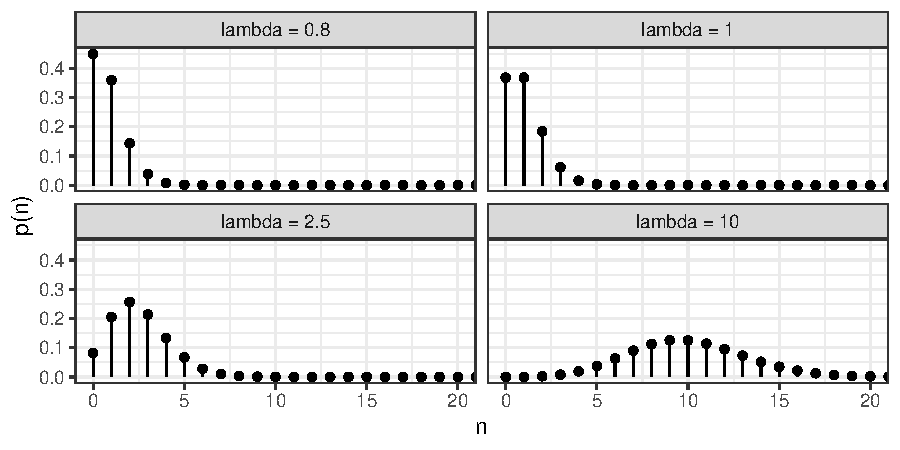
\includegraphics[width=\maxwidth]{figure/plot-poisson-1} 

}



\end{knitrout}
      \label{fig:plot-poisson}
    \end{figure}

  \end{block}
\end{column}

\begin{column}{0.45\linewidth}
  \begin{block}{Distribuzione Gamma}
    $$
    f_Z(z) = \frac{\rho^\alpha}{\Gamma(\alpha)}z^{\alpha-1}e^{-\rho z}, \quad \alpha > 0, \ \rho > 0
    $$
    
    \begin{figure}
      \centering
\begin{knitrout}
\definecolor{shadecolor}{rgb}{0.969, 0.969, 0.969}\color{fgcolor}

{\centering 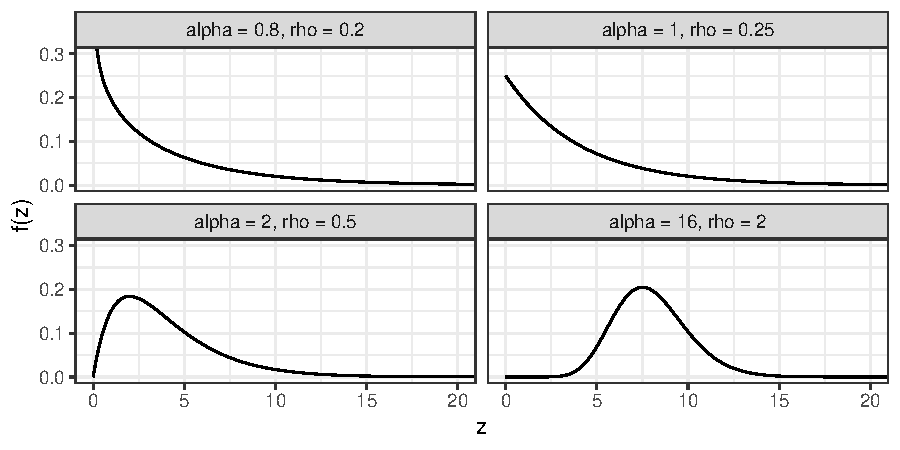
\includegraphics[width=\maxwidth]{figure/plot-gamma-1} 

}



\end{knitrout}
      \label{fig:plot-gamma}
    \end{figure}

  \end{block}
\end{column}

\end{columns}

\end{frame}


%%%%%%%%%%%%%%%%%%%%%%%%%%%%%%%%%%%%%%%%%%%%%%%%%%%%%%%%%%%%%
\begin{frame}
\frametitle{Pricing Tecnico e Commerciale}

\fontsize{9pt}{11pt}\selectfont


\begin{columns}[t, totalwidth=1.02\textwidth]

\begin{column}{0.5\linewidth}
  \uncover<1->{
    \begin{block}{Definizione di Premio}
      \begin{center}
        \begin{tikzpicture}
          \node[text width=4cm, align=left] at (0, 0) (p1) {$P^{(\textrm{risk})}_i=E(S_i)$ \\ $P^{(\textrm{tech})}_i = E(S_i) + E_i$};
          \node[text width=4cm, align=left] at (0, -3cm) (p2) {$P^{(\textrm{tariff})}_i$ \\ $P^{(\textrm{offer})}_i = P^{(\textrm{tariff})}_i - D_i$};
          \draw[black, ->] 
            (-1.5cm, -0.6cm) -- node[right, text width=8cm, align=left]{\footnotesize Altri Caricamenti \\ Vincoli Normativi \\ Commercializzazioni} (-1.5cm, -2.4cm);
        \end{tikzpicture}
      \end{center}
    \end{block}
  }
\end{column}

\begin{column}{0.5\linewidth}
  \uncover<2->{
    \begin{block}{Ottimizzazione del Prezzo}
      
      % \vfill
      % \vspace{0.5cm}
      \vspace{0.8cm}
      
      Si basa su
      \begin{enumerate}
        \item Pricing Tecnico
        \item Aspettativa del Cliente
        \item Strategia di Business
      \end{enumerate}
    
      % \vfill
      \vspace{0.5cm}
      
      Ulteriori modelli
      \begin{itemize}
        \item New Business: Probabilità di Conversion
        \item Rinnovi: Probabilità di Retention
      \end{itemize}

    \end{block}
  }
\end{column}

\end{columns}

\end{frame}





%%%%%%%%%%%%%%%%%%%%%%%%%%%%%%%%%%%%%%%%%%%%%%%%%%%%%%%%%%%%%
\section{Modelli Statistici per il Pricing nelle Assicurazioni Danni}

\begin{frame}
\frametitle{Modello Lineare Generalizzato (GLM)}
\fontsize{9pt}{11pt}\selectfont


\begin{block}{Modello Lineare Generalizzato (GLM)}
  
  Dato $\mathcal{D} = \left\{ (\boldsymbol{x}_1, \omega_1, y_1), \dots,  (\boldsymbol{x}_n, \omega_n, y_n) \right\}$
  
  con $\boldsymbol{y} = (y_1, \dots, y_n)^t$ realizzazione di $\boldsymbol{Y} = (Y_1, \dots, Y_n)^t$.
  
  Assumiamo che:
  \begin{enumerate}
    \item $\boldsymbol{Y} = (Y_1, \dots, Y_n)^t$ siano indipendenti con distribuzione appartenente a una stessa famiglia esponenziale lineare:
    $$f(y_i; \theta_i, \phi, \omega_i) = \exp{\left\{ \frac{\omega_i}{\phi} \left[y_i\theta_i - b(\theta_i) \right] \right\}} \ c(y_i, \phi, \omega_i), \quad y_i\in \mathcal{Y}\subseteq\mathbb{R}$$
    \item $\boldsymbol{x}_i = \left(1, x_{i1}, \dots, x_{ip} \right)^t$ agisca su $Y_i$ tramite il predittore lineare $\eta_i$
    $$\eta_i = \beta_0 + \beta_1 x_{i1} + \beta_2 x_{i2} + \dots + \beta_p x_{ip}$$
    \item $\eta_i$ sia legato a $\mu_i=E(Y_i)$ tramite la funzione legame $g(\cdot)$
    $$g(\mu_i) = \eta_i = \boldsymbol{x}_i^t \boldsymbol{\beta}$$
  \end{enumerate}
\end{block}

\end{frame}



%%%%%%%%%%%%%%%%%%%%%%%%%%%%%%%%%%%%%%%%%%%%%%%%%%%%%%%%%%%%%
\begin{frame}
\frametitle{Stima di un GLM}
\fontsize{9pt}{11pt}\selectfont


\begin{columns}

\begin{column}{0.5\linewidth}
  \uncover<1->{
    \begin{block}{Stimatore di massima verosimiglianza}
      Data la funzione di verosimiglianza
      $$
      \begin{array}{cccc}
        L: & \mathbb{R}^{p+1} \times \Lambda & \longrightarrow & [0, +\infty[ \\
           & \left(\boldsymbol{\beta}, \phi\right) & \longmapsto & f_{\boldsymbol{Y}}(\boldsymbol{y};       \boldsymbol{ \theta}, \phi)
      \end{array}
      $$
  
      Lo stimatore di massima verosimiglianza è:
      $$
      \hat{\boldsymbol{\beta}} = \argmax_{\boldsymbol{\beta}\in\mathbb{R}^{p+1}}{L\left(\boldsymbol{\beta}, \phi; \boldsymbol{y}\right)}
      $$
    \end{block}
  }
\end{column}


\begin{column}{0.5\linewidth}
  \uncover<2->{
    \begin{block}{Devianza}
      La devianza è
      $$
      D(\hat{\boldsymbol{\beta}}, \boldsymbol{y}) =
        -2\phi\left(
        \ell\left(\hat{\boldsymbol{\beta}}, \phi; \boldsymbol{y}\right)
        - \ell_{S}\left(\boldsymbol{\beta}^*, \phi; \boldsymbol{y}\right)
        \right)
      $$
      dove $\ell\left(\hat{\boldsymbol{\beta}}, \phi; \boldsymbol{y}\right) = \log{L\left(\hat{\boldsymbol{\beta}}, \phi; \boldsymbol{y}\right)}$ \newline e $\boldsymbol{\beta}^*$ sono i parametri del modello saturo.
    
      \vspace{0.2cm}
      
      Lo stimatore di massima verosimiglianza può essere ottenuto come:
      $$
      \hat{\boldsymbol{\beta}} = \argmin_{\boldsymbol{\beta}\in\mathbb{R}^{p+1}}{D(\boldsymbol{\beta}, \boldsymbol{y})}
      $$
    \end{block}
  }

\end{column}

\end{columns}


\end{frame}



%%%%%%%%%%%%%%%%%%%%%%%%%%%%%%%%%%%%%%%%%%%%%%%%%%%%%%%%%%%%%
\begin{frame}
\frametitle{titolo}

\end{frame}



%%%%%%%%%%%%%%%%%%%%%%%%%%%%%%%%%%%%%%%%%%%%%%%%%%%%%%%%%%%%%
\begin{frame}
\frametitle{titolo}

\end{frame}



%%%%%%%%%%%%%%%%%%%%%%%%%%%%%%%%%%%%%%%%%%%%%%%%%%%%%%%%%%%%%
\begin{frame}
\frametitle{titolo}

\end{frame}



%%%%%%%%%%%%%%%%%%%%%%%%%%%%%%%%%%%%%%%%%%%%%%%%%%%%%%%%%%%%%
\section{Applicazione Pratica}

\begin{frame}
\frametitle{Titolo di prova capitolo 3}

\end{frame}





\end{document}
